%!TEX root = ../Thesis.tex
\section{Theoretische Grundlagen}


\subsection{Large Language Models}

\subsubsection{Definition und Hintergrund}
Large Language Models (LLMs) bilden einen fundamentalen Baustein für das in dieser Arbeit entwickelte Konzept. Allgemein lassen sie sich als Systeme verstehen, die Verfahren aus den Bereichen Deep Learning und Natural Language Processing (NLP) verwenden, um natürliche Sprache verstehen und generieren zu können. Durch diese Fähigkeit lassen sie sich in den Bereich der Generativen Künstlichen Intelligenz einordnen.

Neuronale Netze bilden hier die technische Grundlage und sind an der Funktionsweise biologischer Gehirne angelehnt. Sie bestehen aus einer großen Anzahl künstlicher Neuronen, die über sogenannte Gewichte miteinander verbunden sind und in mehreren Schichten organisiert werden. Während des Trainings werden diese Gewichte kontinuierlich angepasst, sodass das Modell relevante Muster in den Daten erlernen kann. Auf dieser Grundlage wird die interne Struktur des Netzwerks iterativ optimiert, um möglichst präzise Vorhersagen treffen zu können. Aufgrund dieser Eigenschaften eignen sich neuronale Netze insbesondere für komplexe Klassifikations- und Vorhersageaufgaben.

LLMs stellen eine spezielle Art von Neuronalen Netzen dar, die anhand großer Mengen an Textdaten trainiert werden. Ihre Aufgabe ist es anhand einer Sequenz von sogenannten Token die nachfolgenden Token der Sequenz vorherzusagen. Token können in diesem Zusammenhang ganze Wörter, Wortteile oder Zeichen darstellen. Das Ergebnis des Prozesses ist dabei vollständig davon abhängig, wie das Neuronale Netz seine Gewichte innerhalb des Trainings angepasst hat. 

Das Training besteht allgemein aus 2 Bereichen: dem Pre-Training und dem Fine-Tuning. Beim Pre-Training wird das Modell auf einer sehr großen, meist unstrukturierten Textmenge trainiert – beispielsweise aus dem Internet, Büchern oder wissenschaftlichen Artikeln. Ziel ist es, dem Modell ein breites sprachliches und inhaltliches Grundverständnis zu vermitteln, indem es lernt, Tokens auf Basis vorheriger Sequenzen vorherzusagen. Dieser Schritt ist rechenintensiv und bildet die Grundlage für die späteren Fähigkeiten des Modells.

Im Anschluss erfolgt das Fine-Tuning, bei dem das vortrainierte Modell auf einem kleineren, domänenspezifischen oder aufgabenspezifischen Datensatz weiter trainiert wird. Dadurch kann das Modell gezielt auf bestimmte Anwendungsfälle, Verhaltensweisen oder Kommunikationsstile angepasst werden. Eine verbreitete Methode des Fine-Tunings ist das sogenannte Reinforcement Learning from Human Feedback (RLHF), bei dem menschliche Bewerter die Ausgaben des Modells beurteilen und so dessen Antwortqualität iterativ verbessert wird.

Durch diesen Trainingsprozess und der wiederholten Vorhersage des wahrscheinlich nächsten Token können LLMs zusammenhängende Texte generieren und sprachliche Kontexte berücksichtigen. Es ist jedoch wichtig zu erwähnen, dass es sich dabei um kein echtes tiefgehendes Verständnis von Menschlicher Sprache handelt, sondern lediglich um probabilistische Vorhersagen. Aus diesem Grund kann es vorkommen, dass inhaltlich falsche oder frei erfundene Informationen erzeugt werden. Dieses Phänomen wird als Halluzination bezeichnet. Halluzinationen entstehen insbesondere dann, wenn dem Modell relevante Kontextinformationen fehlen oder Wahrscheinlichkeitsmuster aus den Trainingsdaten zu fehlerhaften Schlussfolgerungen führen.

\subsubsection{Transformer-Architektur}
Ein Großteil der modernen LLMs basiert dabei auf der sogenannten Transformer-Architektur, die 2017 durch Forschende von Google Research in der Arbeit Attention Is All You Need vorgestellt wurde und den Bereich des NLP revolutioniert hat. 

Der Hintergrund dieser Arbeit war es die Limitationen des damaligen State-of-the-Art Ansatzes rekurrenter neuronaler Netze zu Adressieren. Aufgrund einer Sequenziellen Verarbeitung von Textfolgen, konnte das Modell Abhängigkeiten zwischen weit auseinanderliegenden Token nur schwer darstellen, da diese Informationen über lange Sequenzen hinweg immer weiter verloren gingen. Obwohl die Transformer-Architektur aktuell einen fundamentalen Fortschritt in der Leistungsfähigkeit moderner LLMs markiert, sollte erwähnt werden, dass weitere Ansätze zur Verarbeitung natürlicher Sprache existieren. 

Der wesentliche Erfolgsfaktor der Transformer-Architektur bildet der Attention Mechanismus. Dieser erlaubt eine parallele Verarbeitung von Texteingaben, bei der Abhängigkeiten zwischen allen Wörtern berücksichtigt werden. Beispielsweise kann das Wort "Bank" abhängig von dem Kontext in dem es verwendet wird, entweder eine Sitzgelegenheit oder Geldbank darstellen. Durch den Attention-Mechanismus kann das Modell lernen, wie sich die Bedeutung eines Wortes in Abhängigkeit zu dem Kontext verändert. Dadurch sind LLMs, die auf der Transformer-Architektur basieren, in der Lage, Kontextinformationen und semantische Beziehungen auch über längere Textsequenzen hinweg zu berücksichtigen.

\subsubsection{Prompting und Kontextverarbeitung}
Wie das vorherige Kapitel bereits erläutert hat spielt der Kontext in LLMs eine wichtige Rolle. Dieser Kontext wird ihnen über sogenannte Prompts übermittelt. Der Begriff Prompt bedeutet „Aufforderung“ oder „Eingabe“ und beschreibt die textuelle Anweisung, die einem LLM übergeben wird, um eine bestimmte Ausgabe zu erzeugen. Prompts können dabei sowohl einfache Fragen als auch komplexe Anweisungen, Rollenbeschreibungen oder zusätzliche Kontextinformationen enthalten. Die Qualität und Struktur eines Prompts hat einen erheblichen Einfluss auf die Qualität der generierten Antworten.

Im Kontext moderner LLMs wird häufig zwischen verschiedenen Arten von Prompts unterschieden. System-Prompts definieren grundlegende Verhaltensregeln oder Rollen des Modells, beispielsweise die Rolle eines Kundenservice-Chatbots. User-Prompts hingegen enthalten die eigentliche Eingabe des Nutzers. Darüber hinaus können zusätzliche Kontextinformationen bereitgestellt werden, etwa Dokumente, Gesprächsverläufe oder nutzerspezifische Informationen.

Die gezielte Gestaltung solcher Eingaben wird als Prompt Engineering bezeichnet. Ziel des Prompt Engineerings ist es, durch eine geeignete Formulierung der Eingaben die Qualität, Konsistenz und Relevanz der generierten Antworten zu verbessern. Insbesondere im Unternehmenskontext spielt Prompt Engineering eine wichtige Rolle, da dadurch das Verhalten eines Chatbots gezielt an bestimmte Anwendungsfälle angepasst werden kann.

Eine zentrale Herausforderung bei der Kontextverarbeitung von LLMs stellt das sogenannte Kontextfenster dar. Dieses beschreibt die maximale Anzahl an Tokens, die ein Modell gleichzeitig verarbeiten kann. Sämtliche Informationen innerhalb dieses Fensters können vom Modell bei der Generierung einer Antwort berücksichtigt werden. Wird die maximale Größe überschritten, gehen ältere Informationen verloren oder müssen entfernt werden.

Die Größe des Kontextfensters ist insbesondere für dialogbasierte Systeme relevant, da längere Konversationen dazu führen können, dass frühere Informationen nicht mehr berücksichtigt werden können. Dies stellt vor allem für personalisierte Chatbots eine Herausforderung dar, da Nutzerpräferenzen und frühere Interaktionen häufig über längere Zeiträume hinweg relevant bleiben.


\subsection{Chatbots im Unternehmenskontext}
\subsubsection{Definition und Hintergrund von Chatbots}

\subsubsection{Retrieval Augmented Generation}
Unter dem Begriff Vektordatenbanken versteht man ein Datenbanksystem, welches die effiziente Speicherung, Indexierung und Suche hochdimensionaler Vektoren unterstützt. Üblicherweise repräsentieren diese Vektoren die semantische Bedeutung bestimmter Inhalte wie beispielsweise Text, Bild oder Audio. Dabei werden mithilfe von Embedding Modellen aus Inhalten, die in ähnlichen Kontexten auftreten, ähnliche Vektorrepräsentationen erzeugt. Die Ähnlichkeit der Vektoren wird dabei durch Metriken wie der euklidischen Distanz oder dem Skalarprodukt gemessen. Im Gegensatz zu klassischen relationalen Datenbanken ermöglichen Vektordatenbanken die semantische Suche nach inhaltlich ähnlichen Inhalten. Diese Suche basiert meist auf approximativen Verfahren zur Bestimmung der nächsten Nachbarn eines Query-Vektors, wodurch selbst in großen Datenmengen eine effiziente Suche gewährleistet werden kann. 



%\subsection{Personalisierung}

%\subsection{Nutzerpräferenzen}


\subsection{Forschungsansatz und Methodik}
\subsubsection{Design Science Research}
Der wissenschaftliche Forschungsansatz Design Science Research, stellt die Auseinandersetzung mit Artefakten in den Mittelpunkt und ist für diese Arbeit geeignet. Bei der Design Science Research geht es primär darum Probleme, die in einem bestimmten praxisbezogenen Kontext bestehen, strukturiert zu bearbeiten. Das Ziel ist es, eine Verbesserung in dem Problemkontext zu erreichen, indem sich der Forscher mit der Interaktion zwischen Problemkontext und dem Artefakt auseinandersetzt. Hierzu entwickelt der Forscher sogenannte Artefakte. Im Fokus steht dabei nicht das Gestalten völlig neuer Artefakte oder einer Invention. Vielmehr geht es bei der DSR darum das erstellte Artefakt am Ende der Durchführung hinsichtlich seiner Wirksamkeit in Bezug auf das adressierte Problem zu evaluieren.

Artefakte spielen im Bereich der DSR eine zentrale Rolle. Knut Linke beschreibt ein Artefakt als eine „[…] vom Menschen geschaffene Lösung für ein konkretes, praxisbezogenes Problem […]“ (Linke, 2026) und erläutert, dass allein die Entwicklung und Weiterentwicklung von etwas bereits ein Artefakt darstellen kann. In der Praxis kann es sich dabei konkret um Modelle, Konzepte, Softwarearchitekturen oder Prototypen handeln. Allerdings besteht die Anforderung, dass das Artefakt evaluierbar sein muss und vom Forscher problemorientiert untersucht werden kann.

Der Prozess der DSR teilt sich in mehrere Aktivitäten auf, die bei der Durchführung beachtet werden müssen. Diese Arbeit orientiert sich an dem Modell nach Peffers, welches der Abbildung \ref{fig: DSR} entnommen werden kann.

Der Prozess beginnt mit der Problem Identifikation und Motivation. Hier sollte der Forscher das Problem genau beschreiben und die Rahmenbedingungen für das Projekt erläutern. Dabei sollte sowohl aus Empirischer als auch aus Sicht der Praxis eine Relevanz für das Projekt begründet werden. In dieser Phase sollten vor allem Forschungsfragen festgelegt werden, die durch die Durchführung beantwortet werden sollen. Im Anschluss daran müssen aus der Problemstellung die konkreten Ziele abgeleitet werden.

Der nächste Schritt ist es das Artefakt zu erstellen und zu entwickeln. In dieser Phase werden wichtige Design Entscheidungen für das Artefakt getroffen.

Sobald das Artifakt erstellt wurde, muss demonstriert werden, dass es das Problem tatsächlich lösen kann. Es ist also ein Prove of Concept notwendig.

Im letzten Schritt wird die Lösung vor dem Hintergrund des Problemraums und der Zielsetzung evaluiert. Hierzu werden wissenschaftliche Methoden verwendet um die Validität der Lösung empirisch bewerten zu können. Sollte die Evaluation ergeben, dass das Artefakt das Problem und die Ziele nicht lösen kann, ist es notwendig zurück in die Design Phase zu wechseln und den Prozess erneut zu iterieren.

\begin{figure}[hbt]
	\centering
	\begin{minipage}[t]{1\textwidth} % Breite, z.B. 1\textwidth		
		\caption{Design Science Research Method (DSRM) Prozess Modell} % Überschrift
		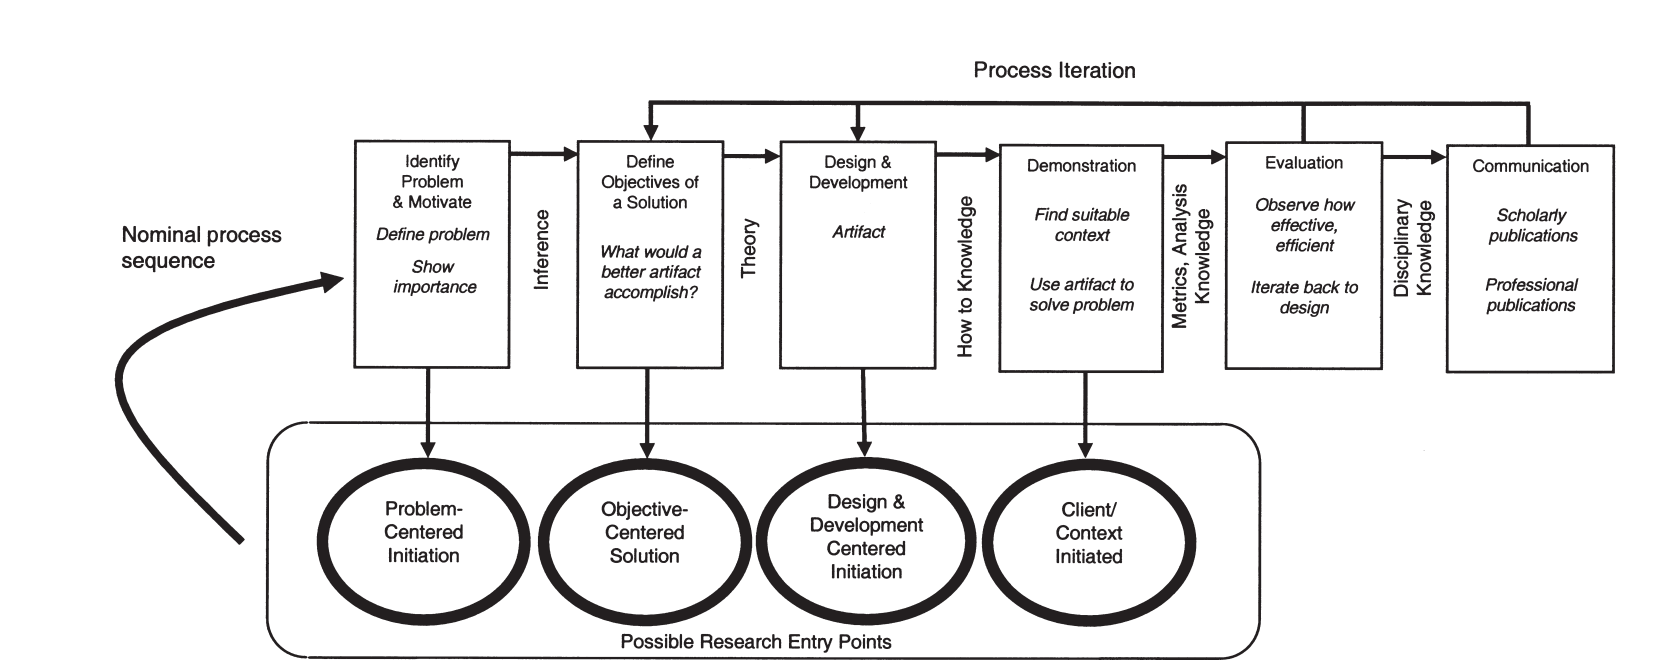
\includegraphics[width=1\textwidth]{img/dsr.png}\\ % Pfad
		\label{fig: DSR}
	\end{minipage}
\end{figure}

\subsubsection{Methodik}


\section{Stand der Forschung}
Die Personalisierung von Chatbots stellt gerade im Unternehmenskontext eine aktuelle Herausforderung dar. Ziel dieses Abschnittes ist es in diesem Zusammenhang aktuelle Techniken und Ansätze aus der Forschung vorzustellen, die sich ebenfalls mit dieser Fragestellung auseinandergesetzt haben.

\subsection{Personalisierte LLMs}
Ein oft behandeltes Thema bilden personalisierte LLMs. Dabei geht es darum LLMs explizit auf die Präferenzen eines Nutzers abzustimmen, sodass diese antworten generieren, die direkt auf eine Person zugeschnitten sind. In der Praxis stellt dies jedoch eine grundlegende Schwierigkeit für Unternehmen dar, da moderne LLMs meist in den Händen der Anbieter sind und sich nicht einfach so neu trainieren lassen. Aus diesem Grund bildet dieser Ansatz, sofern nicht eigene LLMs aufgebaut werden, einen unrealistischen Ansatz für diese Arbeit.

\subsection{Chat Historie}
Ein weiterer Ansatz der in vielen Arbeiten erwähnt wird, ist es die Chat Historie als Kontext in den Prompt zu integrieren. Das LLM könnte in diesem Zusammenhang selbst, die Präferenzen aus der Chat Historie extrahieren und anhand dieser eine Antwort generieren. In Anbetracht der Größe des Kontextfensters für LLMs, zeigen sich dabei jedoch grundlegende Herausforderungen, da die Anzahl an Tokens begrenzt ist. 

\subsection{RAG Ansätze}
Im Jahr 2025 stellten Zhao et al. in ihrem wissenschaftlichen Paper "Do LLMs Recognize Your Preferences? Evaluating Personalized Preference Following in LLMs" einen Benchmark (PrefEval) zur Evaluation der Präferenzverarbeitung in konversationsbasierten LLM-Systemen vor. In dieser Arbeit wurde untersucht, wie gut LLM Modelle Nutzerpräferenzen über längere Konversationen hinweg erkennen, speichern und in Antworten berücksichtigen können.

Die Ergebnisse des Benchmarks zeigen, dass moderne LLMs grundsätzlich in der Lage sind, Nutzerpräferenzen innerhalb von Konversationen zu berücksichtigen. Gleichzeitig zeigt sich jedoch, dass insbesondere die konsistente Verarbeitung von Präferenzen über längere und mehrere Konversationen hinweg weiterhin eine zentrale Herausforderung darstellt. 

Die Ergebnisse des Benchmarks zeigen, dass die Fähigkeit von LLMs zur Berücksichtigung von Nutzerpräferenzen mit zunehmender Gesprächslänge deutlich abnimmt. Während Präferenzen in kurzen Konversationen häufig noch korrekt verarbeitet werden können, sinkt die Genauigkeit bei längeren Dialogen erheblich. Insbesondere Präferenzen, die früh innerhalb einer Konversation genannt wurden, werden von den Modellen häufig nicht mehr zuverlässig berücksichtigt.

%Die Arbeit identifiziert dabei mehrere Problemfelder moderner LLMs im Kontext personalisierter Interaktionen. Dazu zählen unter anderem sogenannte Preference-Unaware Violations, bei denen Nutzerpräferenzen vollständig ignoriert werden, sowie Preference Hallucinations, bei denen Modelle fälschlicherweise Präferenzen ergänzen oder annehmen, die zuvor nicht geäußert wurden. Diese Ergebnisse verdeutlichen, dass große Kontextfenster allein nicht ausreichen, um eine konsistente Personalisierung sicherzustellen. Obwohl relevante Informationen technisch weiterhin im Kontext enthalten sein können, gelingt es den Modellen häufig nicht, diese Informationen zuverlässig abzurufen und in die Antwortgenerierung einzubeziehen.

Die Ergebnisse von PREFEVAL zeigen jedoch auch, dass insbesondere RAG-basierte Ansätze Halluzinationen reduzieren und die konsistente Berücksichtigung von Nutzerpräferenzen verbessern können. Durch den gezielten Abruf relevanter Präferenzinformationen aus externen Speicherstrukturen gelingt es den Modellen besser, frühere Nutzerangaben in späteren Konversationen erneut zu berücksichtigen. Dies ist insbesondere für personalisierte Chatbots im Unternehmenskontext relevant, da Nutzerpräferenzen häufig über längere Zeiträume hinweg konsistent verarbeitet werden müssen.

Externe Retrieval-Mechanismen bilden somit einen vielversprechenden Ansatz, um die Limitierungen kontextbasierter Präferenzverarbeitung moderner LLMs zu adressieren.